\documentclass{beamer}
\usepackage[latin1]{inputenc}
\usepackage{graphicx}
\usepackage{listings}
\usetheme{Warsaw}
\usepackage{tikz}
\usetikzlibrary{trees}

\definecolor{Brown}{cmyk}{0,0.81,1,0.60}
\definecolor{OliveGreen}{cmyk}{0.64,0,0.95,0.40}
\definecolor{CadetBlue}{cmyk}{0.62,0.57,0.23,0}
\definecolor{Red}{cmyk}{0,1,1,0}
\definecolor{Blue}{cmyk}{1,1,0,0}
 
\title{Towards Meaningful Visual Abstraction of Mathematical Notation}
\author{Volker Sorge}
% \author{Davide Cervone \and Peter Krautzberger \and Volker Sorge\thanks{This
%     work was partially supported by the Alfred P. Sloan Foundation.}}
\institute{MathJax Consortium\\
  joint work with Davide Cervone and Peter Krautzberger\\[.5cm]
  This work was partially supported by the Alfred P. Sloan Foundation.}
\date{Washington DC, 13 July 2015}

\begin{document}
\begin{frame}
\titlepage
\end{frame}

\begin{frame}
  \frametitle{Introduction}
  \begin{itemize}
  \item Generation of responsive equations in MathJax
  \item MathJax is a JavaScript library for rendering Mathematics in all browsers
  \item Can take {\LaTeX}, AsciiMath, and MathML as input
  \item Generates browser output, e.g. HTML/CSS, SVG
  \item Standard Maths rendering solution for:
    stackexchange, wordpress blogs, mediawiki, etc.
  \item Internal format is MathML
  \end{itemize}

\end{frame}

\begin{frame}
  \frametitle{Introduction (ctd.)}
  \begin{itemize}
  \item Content has to be displayed well, regardless of the form factor
  \item Responsiveness is ubiquitous
  \item Reading/browsing is more and more dominated by mobile devices
  \item There is a need to work on responsiveness for advanced content
  \item Mathematics is particularly challenging
  \item Authoring is still mainly geared towards static print
  \item Most content is created from {\LaTeX} or AsciiMath which is not ``web friendly''
  \end{itemize}
\end{frame}

\begin{frame}
  \frametitle{Responsive Web Content}
  \begin{itemize}
  \item Responsive design enhances a core feature of HTML: reflow
  \item Originally focused on re-arranging and optimising content
  \item New tools transform the content itself
    \begin{itemize}
    \item cropping images
    \item abstracting icons
    \item modifying tables
    \end{itemize}
  \end{itemize}
\end{frame}

\begin{frame}
  \frametitle{Reflow in Mathematics}
  \begin{itemize}
  \item Combines the properties of text, tables, and graphics into a single problem
  \item Good line-breaking algorithms exist for print
  \item They are often counter-productive on the web
  \item Damage legibility of larger equations beyond repair
  \item Content is usually created with print in mind
    \begin{itemize}
    \item Manual line breaks
    \item arrangements across tabular layout
    \item Tweaks of spacing, etc.
    \end{itemize}
  \item Sensible reflow is much harder to accomplish.
  \end{itemize}
\end{frame}

\begin{frame}
  \frametitle{Responsive Equations}
  \begin{itemize}
  \item Automatic reflow adapting to form factor of display
  \item Intelligent linebreaking
    \begin{itemize}
    \item Don't break in the middle of an expression
    \end{itemize}
  \item Chunking: Abstracting over large elements
    \begin{itemize}
    \item Find meaningful subexpressions
    \end{itemize}
  \item Adapt tabular layout to different screen sizes
  \end{itemize}
\end{frame}

\begin{frame}
  \frametitle{Example}\scriptsize
  \begin{align*}
I_\nu(\nu^{-1},1)
&=\underbrace{\frac{\pi^2}{4}\ln\left(\frac{(1+\nu)^{1+\nu}}{\nu^\nu}
\right)-\frac{7\zeta(3)}{8}\nu}_{\text{Let this be 
C}}+2\int^\frac{1-\nu}{1+\nu}_1\frac{\chi_3(v)}{(1+v)^2}{\rm d}v\\
&=C-\left.\frac{2\chi_3(v)}{1+v}\right|^\frac{1-\nu}{1+\nu}_1+2\int^\frac{1-\nu}
{1+\nu}_1\frac{\chi_2(v)}{v(1+v)}{\rm d}v\\
&=C+(1-\nu)\chi_3\left(\frac{1-\nu}{1+\nu}\right)-\frac{7\zeta(3)}{8}
-\left.{\color{white}{\frac{1}{1}}}2\chi_2(v)\ln(1+v)\right|^\frac{1-\nu}{1+\nu}
_1+\int^\frac{1-\nu}{1+\nu}_1\frac{\ln(1+v)\ln\left(\frac{1+v}{1-v}\right)}{v}{
\rm d}v\\
&=C+(1-\nu)\chi_3\left(\frac{1-\nu}{1+\nu}\right)-\frac{7\zeta(3)}{8}
+2\chi_2\left(\frac{1-\nu}{1+\nu}\right)\ln\left(\frac{1+\nu}{2}\right)+\frac{
\pi^2}{4}\ln{2}\\
&\ \ \ \ 
+\frac{1}{2}\int^\frac{1-\nu}{1+\nu}_1\frac{
\ln^2(1+v)-\ln^2(1-v)+\ln^2\left(\frac{1-v}{1+v}\right)}{v}{\rm d}v
\end{align*}
\normalsize Example of mathematics ``in the wild'' taken from
\href{http://math.stackexchange.com/a/1285149}{math.stackexchange.com}.
\end{frame}

\begin{frame}
  \frametitle{Responsive Equations in MathJax}
  \begin{itemize}
  \item reduce the size of equations by abstracting well-defined parts of
    formulas without obscuring the overall structure of an expression
  \item embedding a semantic structure into the MathML representation underlying
    the rendering process
  \item collapsing mathematically meaningful sub-expressions
  \item exploit information also for linebreaking
  \end{itemize}
\end{frame}

\begin{frame}
  \frametitle{Semantic Enrichment}
  \begin{itemize}
  \item Basis is semantic tree transformation of MathML elements
  \item Uses a rule based implementation implemeneted in a speech rule engine (SRE)
  \item SRE drives math interpretation in ChromeVox (Google) and MathML-Cloud
    (Benetech)
  \item Mainly based on interpreting meaning of symbols.
  \item Rewrite syntax tree into a term tree.
  \end{itemize}
\end{frame}

\begin{frame}
  \frametitle{Semantic Tree Example}
  \[ax^2 + bx + c = 0\] is rewritten from its
Presentation MathML representation into its semantic interpretation:
\lstset{language=html,
    basicstyle=\scriptsize,
    keywordstyle=\bfseries\ttfamily,
    showstringspaces=false,
    otherkeywords={mfenced, open, close, separators, mrow, mi, mo, mn, math, 
      msup, role, parent, children}
}

\begin{minipage}{0.35\textwidth}
\lstinputlisting{quadratic.mml}
% \begin{lstlisting}[language=html]
% \end{lstlisting}
\end{minipage}
\begin{minipage}{0.6\textwidth}
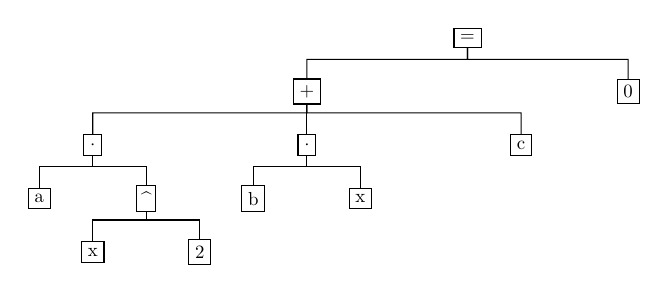
\begin{tikzpicture}[scale=.68, transform shape,
  level 1/.style={sibling distance=4cm,level distance=.8cm}
  ]
  \node[draw] {=}
  [grow via three points={one child at (0,-1.25) and two children at
(-3,-1) and (3,-1)}, edge from parent fork down]
  child {node[draw] {+}[grow via three points={one child at (0,-1) and
two children at (-2,-1) and (2,-1)}, edge from parent fork down]
  child {node[draw] {$\cdot$}[grow via three points={one child at
      (0,-1) and two children at (-1,-1) and (1,-1)}, edge from parent fork down]
    child {node[draw]{a}}
  child {node[draw] {$\,\widehat{}\,$}[grow via three points={one
      child at (0,-1) and two children at (-1,-1) and (1,-1)}, edge from parent fork
    down]
    child {node[draw]{x}}
    child {node[draw]{2}}}
        }
  child {node[draw] {$\cdot$}[grow via three points={one child at
      (0,-1) and two children at (-1,-1) and (1,-1)}, edge from parent fork down]
    child {node[draw]{b}}
    child {node[draw]{x}}
        }
  child {node[draw]{c}}
        }
  child {node[draw] {0}}
  ;
\end{tikzpicture}
\end{minipage}
\end{frame}

\begin{frame}
  \frametitle{Main Heuristics}
  \begin{itemize}
  \item Determine potential function applications,
  \item break up symbol sequences into elided products respecting spaced element,
  \item combine bracketed expressions as much as possible,
  \item recognise scope and nesting of big operators (e.g., sums, integrals),
  \item distinguish tables into matrices, vectors, and case statements,
  \item combine punctuated expressions and determine the meaning of ellipses.
  \end{itemize}
\end{frame}


\begin{frame}
  \frametitle{``Type of Semantic''}
  \begin{itemize}
  \item A shallow interpretation rather than a full blown semantic markup
    language
  \item ``Semantics of display''
  \item Aims to stay faithful to a given notation, without fixing too much
    semantics
  \item Originally developed to deal mainly with K-12 Mathematics
  \item Well honed on some quite horrible MathML input
  \item But it's heuristic, hence with limitations
  \item Useful intermediary step towards further semantic enrichment
  \end{itemize}
\end{frame}


\begin{frame}
  \frametitle{Combining Semantic and MathML}
  \begin{itemize}
  \item MathML is internal representation in MathJax
  \item Embed the semantic interpretation directly using HTML5 data attributes
  \item Alternative view on the MathML element, by providing an orthogonal tree
    structure
  \item No exposure to the outside yet
  \item Some issues with embedding:
    \begin{itemize}
    \item Adds some \texttt{mrow} elements, invisible elements.
    \item Collapsed elements have to be noted explicitly.
    \item Special cases for \texttt{mfenced}, \texttt{mmultiscripts}
    \end{itemize}
  \end{itemize}
\end{frame}


\begin{frame}
  \frametitle{Rendering Enhancements}
  \begin{itemize}
  \item Initial enrichment can already lead to enhanced rendering
  \item E.g. breaking up single \texttt{mrow}s with stretchy characters:\\
    Before

    \[ 
      \biggl\vert \tau_0 \biggr\vert = \biggl\vert  \sum_{m} \bigg(a_b + b_m\bigg) 
      \bigg\vert 
    \]
    After
    \[ 
      \left\vert  \tau_0 \right\vert = \left \vert \sum_{m} \left(a_b + b_m\right) 
      \right\vert 
    \]
  \item Similar effects for line breaking
  \end{itemize}
\end{frame}


\begin{frame}
  \frametitle{Responsive Equations}
  \begin{itemize}
  \item Targets ``casual reading'', i.e. reader browses without the need for
    full details
  \item Collapse and re-arrange sub-expressions on small screens to provide the
    reader with a meaningful overview of the expression 
  \item Realise an interface for exploration of collapsed equations.
  \end{itemize}
\end{frame}

\def\collapse#1{\textcolor{blue}{\ensuremath{\mathord{\blacktriangleleft}\mathord{#1}
\mathord{\blacktriangleright}}}}

\begin{frame}
  \frametitle{Exploring Equations}
  \begin{minipage}{.49\linewidth}
    \begin{itemize}
    \item Subexpressions over a certain complexity are hidden
    \item Complexity measure mainly aims at shortening an equation
    \item Collapsed parts are represented by a simple meaning Unicode
      construction, \collapse{X}.\\
      E.g., \collapse{()},\collapse{f()},\collapse{+},\collapse{\raise2pt\hbox{$\sqrt{}$}\,}
    \end{itemize}
  \end{minipage}
  \begin{minipage}{.49\linewidth}
   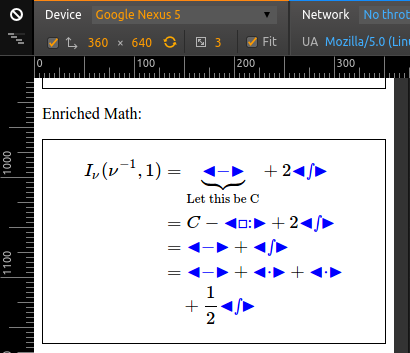
\includegraphics[width=1\textwidth]{./ex_long_collapse.png}
 \end{minipage}
 
\end{frame}

\begin{frame}
  \frametitle{Exploring Equations (ctd.)}
  \begin{minipage}{.49\linewidth}
    \begin{itemize}
    \item standard \texttt{maction} elements on collapsible parts of equation
    \item \texttt{maction toggles} to show or hide those parts
    \item exploration via expanding and collapsing nested layers of the equation
    \end{itemize}
  \end{minipage}
  \begin{minipage}{.49\linewidth}
    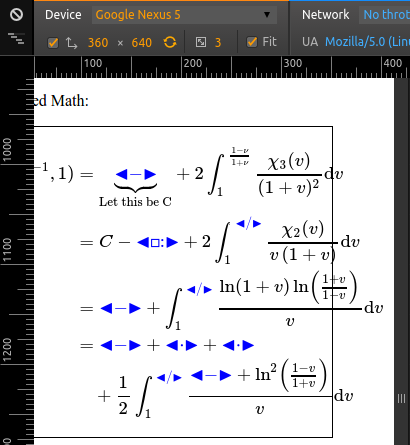
\includegraphics[width=1\textwidth]{./ex_long_collapse2.png}
  \end{minipage}
\end{frame}


\begin{frame}
  \frametitle{Discussion}
  \begin{minipage}{.5\linewidth}
    \begin{itemize}
    \item UX is not ideal:
      \begin{itemize}
      \item collapse can be accidentally triggered
      \item expansion via single steps only
      \end{itemize}
    \item Complexity measure mainly tries to determine visual layout size.
      Other measures could capture a notion of interestingness, etc.
   \item Display vs exploration
      \begin{itemize}
      \item Sometimes collapsed parts do not save any more space.
      \item Stepwise exploration might still be interesting.
      \end{itemize}
    \end{itemize}
  \end{minipage}
  \begin{minipage}{.4\linewidth}\scriptsize
    \begin{align*}
      \frac{1}{\collapse{\cdot}} &= 1 + \collapse{/}\\
      \frac{1}{\Bigl(\collapse{\surd}-\phi\Bigr)
      e^{\frac25\pi}} &=
                        1+\frac{e^{-2\pi}}
                        {1+\collapse{/}}\\
      \frac{1}{\Bigl(\collapse{\surd}-\phi\Bigr)
      e^{\frac25\pi}} &=
                        1+\frac{e^{-2\pi}}
                        {1+\frac{e^{-4\pi}}
                        {1+\collapse{/}}
                        }\\
      \frac{1}{\Bigl(\sqrt{\phi\sqrt{5}}-\phi\Bigr)
      e^{\frac25\pi}} &=
                        1+\frac{e^{-2\pi}}
                        {1+\frac{e^{-4\pi}}
                        {1+\collapse{/}}
                        }\\
      \frac{1}{\Bigl(\sqrt{\phi\sqrt{5}}-\phi\Bigr)
      e^{\frac25\pi}} &=
                        1+\frac{e^{-2\pi}}
                        {1+\frac{e^{-4\pi}}
                        {1+\frac{e^{-6\pi}}
                        {1+\collapse{/}}}}
      \\
      \frac{1}{\Bigl(\sqrt{\phi\sqrt{5}}-\phi\Bigr)
      e^{\frac25\pi}} &=
                        1+\frac{e^{-2\pi}}
                        {1+\frac{e^{-4\pi}}
                        {1+\frac{e^{-6\pi}}
                        {1+\frac{e^{-8\pi}}
                        {1+\ldots} } } }
    \end{align*}
  \end{minipage}
\end{frame}

\begin{frame}
  \frametitle{Accessiblity Unit}
  \begin{itemize}
  \item Exploit semantic information directly for voicing of equations
  \item Use collapsed equations for intelligent summarisation
  \item Interactive exploration with respect to current maction units
    for improved chunking
  \item {Further assistive technology support}
 \begin{itemize}
  \item Make information available for other AT systems
  \item Push data attributes into the actual DOM content as micro data that can
    be exploited by some AT and  Accessibility APIs
  \end{itemize}

  \end{itemize}
\end{frame}



\begin{frame}
  \frametitle{Conclusion}
  \begin{itemize}
  \item Responsive equations with collapsing and enhanced line breaking
  \item Semantics is shallow but effective
  \item Good results with mathematics in the wild
  \end{itemize}

  \begin{itemize}
  \item Work on breaking up tables and tabular alignment.
  \item Intelligent accessibility via summarisation etc.
  \item Support of assistive technology
  \end{itemize}

  Demo this evening.
\end{frame}

\begin{frame}
  \frametitle{Web References}


  \begin{itemize}
  \item Demo:
    \begin{itemize}
    \item \url{http://mathjax.github.io/MathJax-RespEq/Semantics-Lab/Struik.html}
    \item \url{http://mathjax.github.io/MathJax-RespEq/Semantics-Lab/Semantics-Lab-TeX.html}
    \item \url{http://mathjax.github.io/MathJax-RespEq/Semantics-Lab/Semantics-Lab-TeX-linebreaking.html}
    \end{itemize}
  \item Systems:
    \begin{itemize}
    \item \url{https://github.com/mathjax/MathJax/}
    \item \url{https://github.com/mathjax/MathJax-RespEq/}
    \item \url{https://github.com/zorkow/speech-rule-engine/}
    \item \url{https://github.com/mathjax/MathJax-node/}
    \end{itemize}
  \end{itemize}
\end{frame}

\end{document}

%%% Local Variables:
%%% mode: latex
%%% TeX-master: t
%%% End:
